% \documentclass[preprint]{kcc}
\documentclass{kcc}

%%%%%%%%%%%%%%%%%%%%%%%%%%%%%%%%%%%%%%%%%%%%%%%
% include additional packages you need to use
%%%%%%%%%%%%%%%%%%%%%%%%%%%%%%%%%%%%%%%%%%%%%%%
% graphic, float package
\usepackage{graphicx}		% for setting images
\usepackage{float}			% for float objects
\usepackage{subfloat}		
\usepackage{subfigure}		% for adding several figures in a figure environment
\usepackage{lscape}			% for landscape type images or tables
\usepackage{url}		

\usepackage{enumitem}

% for compact section title spacing
% \usepackage[compact]{titlesec}


% mathmetical presentation
\usepackage{gensymb}
\usepackage{amsmath}
\usepackage{amssymb}
\usepackage{amsthm}
\usepackage{exscale}
\usepackage{textcomp}		% extra symbols


% for circled number
\newcommand{\cl}[1]{\textcircled{\scriptsize #1}}


% package for using algorithmic presentation
\usepackage{algorithmic}
\usepackage{algorithm}
% customize algorithmic environment
\renewcommand{\algorithmicrequire}{\makebox[40px]{\hfill\textbf{Input :}}}
\renewcommand{\algorithmicensure}{\makebox[40px]{\hfill\textbf{Output :}}}

% array and table presentation
\usepackage{array}
\usepackage{tabulary}
\usepackage{multirow}
\usepackage[table]{xcolor}
\usepackage{ctable}
\usepackage{booktabs}		% for typesetting tables at the level of publication		
							% do not use vertical rule
							
% set title, author, abstract
\title{대학수학능력시험 생명과학 1 문제의 유형 분류를 위한 기계학습의 적용}
\author{
송하윤$^{\circ}$, 심현섭\\
홍익대학교 컴퓨터공학과\\
hayoon@hongik.ac.kr, nospacethere@gmail.com
}
\engtitle{An Application of Machine Learning for the Classification of Biology 1 Problems of the Korean CSAT}
\engauthor{
Ha Yoon Song, Hyeon Seop Shim\\
DePartment of Computer Engineering, Hongik University, Seoul, Korea\\
}
\abstract{
대한민국의 대학수학능력시험 중 생명과학 문제들의 유형을 5개로 분류하기 위하여, 기계학습 기법 기반의 해법을 제시한다. 생명과학 문제를 5개의 주요 카테고리로 자동으로 분류하기 위하여 합성곱신경망(Convolutional Neural Network, CNN) 기반의 모델과 하이퍼파라미터 집합을 제시한다. 각 문제의 첫 문단을 Tokenizer와 Padding 작업 과정을 거쳐 5,000개의 문제 데이터를 전처리하는 단계를 거친다. 모델 개발 단계에서는 그리드-서치 알고리즘 기법을 이용하였으며, 하이퍼파라미터를 인위적으로 설정하여 각각의 구간으로 나눈다. 시험 평가 단계에서는 Train-Validation-Test Split을 6:2:2의 비율로 적용하여 하이퍼파라미터 6개 각각의 구간으로부터 파라미터 값이 서로 다른 729개의 하이퍼파라미터 조합을 생성한 후 각각의 예측 정확도를 평가하게 된다. 그 다음에는, Test-Set 평가에서의 예측 정확도가 높은 상위 5개의 모델을 선별한 후, 그 조합들에 대한 모집단의 정확도를 구하기 위해 샘플 모델들을 각각 100개씩 만들어 표준정규분포로 정확도를 분석하였다. 대체로 조합들은 유의 수준 0.05 내에서 93.71\% 의 정확도를 보여준다. 최종적으로, 각 문제들의 텍스트를 인식하여 정해진 5개의 유형에 맞게 자동 분류할 수 있는 기계학습 기법을 구현하였다.
%This study presents a machine learning solution for automatically classifying Biology 1 questions from the Korean College Scholastic Ability Test into five main categories. To achieve this, 5,000 Biology 1 question data were preprocessed using a tokenizer and padding process, and a model based on Convolutional Neural Networks (CNN) was developed. The model's hyperparameters were optimized using a grid-search algorithm, and the text dataset was split into Train-Validation-Test with a ratio of 6:2:2, generating 729 hyperparameter combinations. The top five models with the highest prediction accuracy in the test set were selected, and when these models were regenerated 100 times each and analyzed for prediction accuracy using a standard normal distribution, they showed a high average accuracy of 93.71% at a significance level of 0.05. This research demonstrates the effectiveness of a machine learning technique for the automatic classification and evaluation of Biology 1 questions in the college entrance exam, thus expanding the possibilities for the application of machine learning in the field of education.
}
\begin{document}

\maketitle


\section{서 론}
대한민국의 국가 시험 중 대학수학능력시험은 대학을 진학하기 위한 수험생들의 마지막 관문이다. 
여러 교육 산업들은 수험생들이 시험 대비를 할 수 있게 도와주면서 새로운 사업 모델, 특히 AI 응용 관련 시장을 모색하기 위해, 
학습자 개개인의 요구에 맞춤화된 교육 제공을 목적으로 LMS(Learing Management System)\cite{cite:lms}에 AI를 부가 도입하는 등, 전례에 없었던 기능을 크게 확장하고 있다.
특히 사교육 시장에서는 학생 소비자들에 문제 풀이 및 해설에 도움을 주고자, 각자의 교육 플랫폼에 도입시킬 여러 과목들의 기초적인 유형 분류 모델 개발에 연구하고 있다.

\cite{cite:handwriting1}에서는
현재 수준의 교육용 AI 중 유형 분류 모델은 수학의 수식 인식\cite{cite:MathFormulaRecognition}을 통한 수학 과목 문제 유형 분류 모델이 개발되었으나, 
나머지 과목들 중 텍스트 중심 형태로 이루어진 문제들을 유형 분류하는 모델 개발 연구가 집중적으로 이루어진 사례는 거의 드물다.

이 연구에서는 딥러닝 분야 중 CNN(Convolutional Neural Network)을 적용하여 유형 분류 모델을 제시한다. 문제 데이터를 넣으면 텍스트 전처리 과정을 통해 생명과학 1 유형 5개 중 하나로 분류되는 모델을 개발한다. 문제 데이터는 생명과학 5,000개의 문제에서 각각 첫 번째 문단을 가져온 텍스트 형식으로 이루어져 있으며, 정규표현식을 통한 특수문자 제거 등 복잡한 전처리 과정을 거치지 않은 원본 형태이다.
데이터 전처리 단계에서는 토크나이저(Tokenizer) 작업과 패딩(Padding) 작업 과정을 거치게 된다. 전처리된 데이터들은 모두 Train Set, Validation Set, 그리고 Test Set으로 나누게 된다.

모델 개발 단계에서는 그리드-서치(Grid-Search) 알고리즘 기법을 이용하기 위하여 총 6개의 하이퍼파라미터 독립 변수들(Input\_dim, Output\_dim, Epochs, Conv1D\_filter, Conv1D\_kernel, Density)을 조합, 총 729개의 서로 다른 하이퍼파라미터 집합을 생성하게 된다. 
평가 시험 단계에서는 각 모델들의 정확도로부터 하이퍼파라미터 구간에 따른 평균-정확도를 구하여 분석하게 된다. 그 다음, 정확도가 높은 상위 5개의 하이퍼파라미터 조합을 각각 100개씩 생성하여 Z-분포의 신뢰도 90\%, 95\%, 99\%에 따른 정확도를 분석하게 된다.

\section{본문}
다양한 모델중 CNN을 이용하였을 때의 기초 실험 결과가 가장 우수하였고, 실행 속도 또한 높았다. 따라서 본 논문에서는 CNN 기법을 적용한다. 일반적으로, CNN을 적용한 모델은 이미지를 인식하여 패턴을 찾는 분류 모델\cite{cite:TextRecognition1}로, 이미지 데이터를 처리할 때 2차원 구조에서 이미지의 공간 정보\cite{cite:cui2024deep}를 유지하여 패턴을 인식한 다음 Fully Connected Layer에 넣는 것으로 알려져있다. 하지만 텍스트 데이터를 처리할 때는 입력 데이터를 1차원 배열 형태로 한정하여 문장 내 Sequence 패턴\cite{cite:textClassification1}을 찾는다. 주로 1차원 컨볼루션 망을 이용하여 각 단어나 문자의 순서 사이에서 패턴을 찾게 되며 임베딩 작업을 통해 실수 벡터로 변환해 문맥적 특징을 추출하고 학습하게 된다.

텍스트로부터 Word2Vec을 통한 전처리 작업(Embedding)\cite{cite:zhang2024teleclass}을 거치기도 하지만, 해당 작업이 꼭 모델의 성능 향상에 도움을 주진 않는다는 연구 결과\cite{cite:word2vec}가 있어, 복잡한 전처리 과정을 진행하지 않는다.\cite{cite:jiang2024quick}

먼저, 텍스트를 숫자 차원으로 변환하기 위해서는 두 가지 과정의 전처리 작업을 거치게 된다.

토크나이저(Tokenizer) 단계에서는 텍스트 문장을 작은 단위인 'Token'\cite{cite:OnlineTokenizer}으로 나눈 후, 각 토큰에 대해 정수 인덱스 할당하는 과정\cite{cite:TokenizerforCNN}을 거치게 된다. 이 과정은 단어 대신 인덱스로 교체하여 모델을 학습시키기 위한 데이터로 변환시키는 데에 목적이 있다.

패딩(Padding) 단계에서는 전 단계에서 만들어진 시퀸스 데이터(Sequence Data)를 일정하게 길이를 맞추는 작업\cite{cite:Lopez-delRio2020EffectOfSequencePadding}을 하게 된다.

이로써, 첫 레이어에서는 저차원 벡터로 임베드\cite{cite:Reddy2020EffectOfPadding}하게 되며, 그 다음 레이어(Hidden Layer)에서는 여러 사이즈의 필터를 통해 벡터에 대한 합성곱 변환\cite{cite:IntroductionforCNN}을 진행하게 된다.

\begin{figure}[!ht]
\centering
\includegraphics[width=0.4\textwidth]{figs/fig_layout}
\caption{CNN 모델 구조 모식도}
\label{fig:example1}
\end{figure}
\index{figure}

실험 모델에 들어갈 데이터는 한국의 대학수학능력시험 과목 중 생명과학 1 문제들을 참조하였으며, 총 5,000 문제의 텍스트 데이터와 5개의 클래스를 준비하였다. 모델 내부로부터 나온 반환값의 구조가 그림~\ref{fig:example1}에 예시로 나타나 있다. 분류되는 유형은 5개 중 하나이므로 모델에서 반환되는 값은 길이가 5이면서 모두 0으로 채워진 배열에서, 가장 확률이 높다고 추론된 배열 인덱스에 1을 부여한다. 즉, 각 문제들은 One-Hot Encoding 형식으로 5개의 유형 중 하나를 결정하게 되며, Json 파일 형태로 일관되게 저장한다. 이러한 데이터로 학습된 모델들은, 후에 새로운 텍스트 데이터나 기존에 학습된 텍스트 데이터가 들어올 경우 5개의 단원 중 하나를 예측하게 된다.

\begin{figure}[!ht]
\centering
\includegraphics[width=0.4\textwidth]{figs/dataFigure}
\caption{데이터 구조 모식도}
\label{fig:example1}
\end{figure}
\index{figure}

\subsection{관련 연구}

\subsubsection{Grid-Search Algorithm}
성능(정확도)이 좋은 모델을 개발하기 위해, 개발 모델의 변수들에 인위적으로 정적인 값들을 대입하여 탐색하는 기법\cite{cite:grid}을 이용한다.
해당 모델 개발에서 하이퍼파라미터는 총 6개로, \ref{models}에 나타난 독립 변수들(Input\_dim, Output\_dim, Epochs, Conv1D\_filter, Conv1D\_kernel, Density)을 각각 세 구간으로 나누어 여러 조합의 모델을 탐색하게 된다.

\subsubsection{Train-Validation-Test Split}
기존에는 모델의 성능 평가를 위해 데이터셋 분리는 Train-Test Split을 8:2로 선택 하였으나\cite{cite:split}로 진행됐으나, 해당 모델의 개발 과정에서 좀 더 면밀한 관찰을 위해 Train-Validation-Test Split을  6:2:2로 제안한다.
이러한 데이터셋 분리가 도움이 되는 이유는 Validation-Set과 Test-Set 간의 차이가 있다. Validation-Set에서는 훈련시킨 데이터에 대해 모델의 정확도를 검증하게 된다. 반면에 Test-Set에서는 훈련되지 않은 데이터에 대해 모델의 정확도를 검증하기에 중간 검증 과정에서 과적합 영역\cite{cite:SplittingData}을 쉽게 찾을 수 있다. 따라서 모델의 실제 성능에 대한 추정치(예측 정확도)를 분석할 수 있으며, 각 상황에 따른 견고성을 고려해 볼 수 있다.

\subsubsection{Z-분포(표준정규분포)}
실험에서 만들어진 모델들은 예측 정확도에 대한 안정성이 검증된 모델들이 아니기 때문에, 어느 정도의 표준적인 평가 척도가 필요하다. 따라서 샘플 모델들의 예측 정확도 분석에 대해서는 Z-분포(표준정규분포) 기법을 제안한다.
표본 개수가 약 30개 또는 100개 이상으로 충분할 때, 중심극한정리\cite{cite:CentralLimit}에 의거하여 독립적인 확률변수 X에서 어떠한 값 분포에 대한 평균은 정규분포에 가까워진다고 볼 수 있다\cite{cite:Probability}. 따라서 두 개의 매개변수 중 평균과 표준편차에 의해 그 모양이 결정된다.

\begin{eqnarray}
z = \frac{(x - \mu)}{\sigma / \sqrt{N}}
\end{eqnarray}

${z}$는 데이터의 포인트가 평균으로부터 얼마나 떨어져 있는지를 나타내는 표준편차 단위이다.
${x}$는 각 개별 데이터의 포인트가 된다.
$\mu$와 $\sigma$는 각각 모집단에서의 모든 데이터 포인트의 평균값과 표준편차를 말한다.
${N}$은 모집단을 구성하는 샘플 모델의 개수를 말한다.
무작위로 생성된 데이터셋들로부터 동일한 하이퍼파라미터를 가진 샘플 모델들을 최대한 많이 생성하여 모집단 하이퍼파라미터 조합의 정확도를 구하기 위해, 샘플 모델들의 평균-정확도와 표준편차를 구하는 것이다. 이러한 값들을 구한 후 신뢰 구간을 3개로 나누어, 각각 90\%, 95\%, 99\%에 대한 정확도 분포를 구하게 된다.



\subsubsection{Categorical Crossentropy}
다중 클래스 분류 문제에서 널리 사용되는 손실 함수\cite{cite:CategoricalCrossentropy} 중 하나이며, 실제 클래스 레이블과 모델의 예측 정확도 확률 분포 간의 차이를 측정한다. 주로 Softmax 활성화 함수\cite{cite:softmax}와 함께 사용된다. 각 클래스들의 확률 분포의 합은 1이 되며, 레이블이 1인 클래스만 로그 확률을 계산하고 나머지는 무시한다.

\begin{eqnarray}
H(y, \hat{y}) = -\sum_{i} y_i \log(\hat{y}_i)
\end{eqnarray}

${H}$는 교차 엔트로피의 손실 함수를 나타내는 함수이다.
${y}$는 실제 레이블의 i번째 클래스에 대한 값이며, 주로 One-Hot Encoding 형식으로 표현된다.
$\hat{y}_i$는 모델에 의해 예측된 i번째 클래스에 대한 확률이다.
손실 함수의 계산은 레이블이 1인 클래스에 대해서만 수행되며, 예측된 확률의 로그 값에 실제 레이블 값을 곱하여 모든 클래스에 대해 합산하게 된다. 따라서 최종 손실 값은 양수가 나오게 되며, 낮은 값일 수록 모델이 제시한 예측이 정확하다는 것을 알 수 있다.

\subsection{모델 생성 및 하이퍼파라미터 조합}
\label{models}

이 영역에서는 하이퍼파라미터 조합에 대한 시험 평가를 두 단계에 걸쳐서 하게된다.
하이퍼파라미터는 총 6개로, Input\_dim, Output\_dim, Epochs, Conv1D\_filter, Conv1D\_kernel, Density으로부터 구간을 설정한다.
\begin{itemize}[itemsep=0pt,Parsep=0pt]

\item Input\_dim은 모델이 입력 데이터를 받아들일 때 나타나는 텍스트 형태나 차원을 나타낸다.
\item Output\_dim은 합성곱 신경망을 통과하여 나오는 예측값이나 분류 결과의 차원을 말한다.
\item Epoch는 전체 데이터 세트에서 학습 과정을 거치는 횟수를 말하는데, 일반화 과정을 거치는 작업을 말한다.
\item Conv1D\_filter는 1차원 합성곱 계층에서 사용되는 필터를 말한다. 이는 특징 추출\cite{cite:Convoultional}을 하는 데에 사용되는 학습 가능한 필터의 총 개수를 말한다.
\item Conv1D\_kernel은 1차원 합성곱 계층에서 사용되는 필터의 크기를 말한다. 이는 커널의 크기가 합성곱 필터로부터 입력 데이터를 어느 범위로 처리할지를 말한다.
\item Density는 Dense Layer나 Fully Connected Layer의 층에 있는 뉴런의 수를 말한다. 모든 입력을 각 출력에 연결을 하게 되며, 각 연결의 가중치를 학습하게 된다.
\end{itemize}

\subsubsection{Grid-Search Test}
첫 번째 단계는, 전처리 단계에서 생성된 729개의 조합을 각 하이퍼파라미터 구간의 평균-정확도를 분석하게 된다.
그리드-서치 알고리즘 기법을 통하여 총 6개의 하이퍼파라미터 독립 변수들(Input\_dim, Output\_dim, Epochs, Conv1D\_filter, Conv1D\_kernel, Density)을 이용하여 729개의 조합들로부터 Validation-Set 평가에서의 평균 정확도와 표준편차를, Test-Set 평가에서의 평균 정확도와 표준편차를 나타낸 것이다.

이 영역에서는 텍스트 유형 분류를 위한 모델 개발 단계로, 5,000 개의 전처리된 데이터를 각각 Train-Validation-Test Split으로 나누어 각각 6:2:2로 무작위 Data Set\cite{cite:SimpleRandeomSampling}을 생성하게 된다. 각 조합을 통해 모델이 만들어질 때마다 모든 Data Set들은 다시 초기화\cite{cite:SamplingMethods}되며, 일련의 작업들을 다시 거치게 된다.

모델 개발 중 Optimizer\cite{cite:OptimizingforCNN}는 TensorFlow의 Keras 모델로부터 Adam Optimizer로 설정하였다. Adam Optimizer는 1차 기울기 기반 최적화를 위한 방법으로, Stochastic Objective Functions\cite{cite:kingma2017adam}를 따른다. 학습되는 데이터도 적은 만큼, Learning\_rate를 평균적인 수치인 0.001로, Complie 함수는 'Categorical\_Crossentropy'를 사용한다.

\subsubsection{Standard-Normal-Distribution Test}
두 번째 단계에서는, 첫 번째 실험에서 구현된 729개의 조합 중 정확도가 높은 상위 5개 모델을 택하여, 하이퍼파라미터가 같은 각각의 샘플 모델 100개씩 무작위로 생성하여 모델 평가를 진행하며 표준정규분포\cite{cite:NormalDistribution}에 따라 Z-분포의 신뢰 구간(90\%, 95\%, 99\%)에 따른 정확도의 오차 범위를 분석하게 된다.

\subsection{모델 평가}
이 영역에서는 각각의 테스트에서 만들어진 시험 모델에 대한 평가 지표를 제시한다.
실험 환경은 모두 Google Colab~\cite{cite:google}에서 지원하는 Python3 Google Compute Engine BackEnd 내에서 TPU를 이용하였다.
시스템 RAM은 12.7GB로, 디스크 크기는 107.7GB로 설정하였다.

\subsubsection{최적화된 하이퍼파라미터 검색}
\label{search}
이 실험에서는 6개의 하이퍼파라미터를 각각 세 구간으로 나누어 각각의 조합을 생성하였다.
\begin{table}[!ht]
\centering
\setlength{\belowcaptionskip}{5pt}
\caption{HyperParameter}
\label{tab:HyperParameter}
\begin{tabular}{@{}lcccc@{}} 
\toprule
{\bfseries Parameter} & \multicolumn{3}{c}{\bfseries Value} \\
\midrule
Input\_dim  & 100 & 150 & 200 \\
Output\_dim  & 200 & 300 & 400 \\
Epochs & 5 & 10 & 15 \\
Conv1D\_filter & 64 & 96 & 128 \\
Conv1D\_kernel & 5 & 10 & 15 \\
Density & 64 & 96 & 128 \\
\bottomrule
\end{tabular}
\end{table}

표 \ref{tab:HyperParameter} 에서는 앞서 'Grid-Search Test'에서 실험하고자 진행한 하이퍼파라미터를 6개를 Category에, 그 다음은 설정된 값을 Value로 나타낸 모습이다. 각 카레고리에는 3개의 변수값이 주어지므로, 총 729개의 서로 다른 조합이 나오게 된다.

6개의 하이퍼파라미터를 세 구간으로 나누었기에 다음 테이블들의 범례에서 'Par'는 설정된 구간 값을 의미하고 'N'은 그 구간에 설정된 실험 모델의 총 개수를 의미한다. 

나머지 부분에서는, 각 구간에 존재하는 243개의 하이퍼파라미터 집합에 대한 예측 정확도 평균과 표준편차를 나타내게 된다. Train-Validation-Test Split을 거친 상태에서 하이퍼파라미터들을 평가하게 됐으므로, Validation과 Test 부분으로 나누어 예측 정확도 평균(\%)과 표준편차를 구하게 된다. Validation에서의 평균과 표준편차는 각각 'Avg\_v'와 'StDev\_v'로 표기하고, Test에서의 평균과 표준편차는 'Avg\_t'와 'StDev\_t'로 표기하였다.

\begin{table}[!ht]
\centering
\setlength{\belowcaptionskip}{5pt}
\caption{Input\_dim}
\label{tab:Input_dim}
\begin{tabular}{@{}lcccc@{}} 
\toprule
{\bfseries Par (N)} & 100 (243) & 150 (243) & 200 (243) \\
\midrule
Avg\_v  & 98.41 & 99.02 & 99.43 \\
Avg\_t  & 89.88 & 91.70 & 93.56 \\
StDev\_v & 0.79 & 0.50 & 0.34 \\
StDev\_t & 0.84 & 1.07 & 0.99 \\
\bottomrule
\end{tabular}
\end{table}

표 \ref{tab:Input_dim}에서는 하이퍼파라미터 중 Input\_dim을 100, 150, 200으로 구간을 나누어 조합을 생성한 모습이며, 구간 값이 커질수록 모델의 예측 정확도가 크게 향상됨을 보인다. 이는 더 큰 Input 임베딩 차원을 사용할 때, 모델이 학습 데이터를 자세히 습득하여 더 나은 결과를 보이는 것을 알 수 있다.

\begin{table}[!ht]
\centering
\setlength{\belowcaptionskip}{5pt}
\caption{Output\_dim}
\label{tab:Output_dim}
\begin{tabular}{@{}lcccc@{}} 
\toprule
{\bfseries Par (N)} & 200 (243) & 300 (243) & 400 (243) \\
\midrule
Avg\_v  & 98.91 & 98.98 & 98.97 \\
Avg\_t  & 91.68 & 91.71 & 91.75 \\
StDev\_v & 0.76 & 0.69 & 0.67 \\
StDev\_t & 1.79 & 1.76 & 1.82 \\
\bottomrule
\end{tabular}
\end{table}


표 \ref{tab:Output_dim}에서는 하이퍼파라미터 중 Output\_dim을 200, 300, 400으로 구간을 나누어 하이퍼파라미터 후보군을 생성한 모습이며, 구간 값에 따라 모델의 예측 정확도가 비례하는 현상은 나타나지 않는다.

\begin{table}[!ht]
\centering
\setlength{\belowcaptionskip}{5pt}
\caption{Epochs}
\label{tab:Epochs}
\begin{tabular}{@{}lcccc@{}} 
\toprule
{\bfseries Par (N)} & 5 (243) & 10 (243) & 15 (243) \\
\midrule
Avg\_v  & 98.64 & 99.07 & 99.16 \\
Avg\_t  & 91.57 & 91.69 & 91.88 \\
StDev\_v & 0.89 & 0.56 & 0.49 \\
StDev\_t & 1.82 & 1.83 & 1.71 \\
\bottomrule
\end{tabular}
\end{table}

표 \ref{tab:Epochs}에서는 하이퍼파라미터 중 Epoch를 5, 10, 15으로 구간을 나누어 조합을 생성한 모습이며, 구간 값에 따라 모델의 예측 정확도가 미세하게 향상된 것을, 표준편차 또한 약간 줄어드는 것을 보이고 있다.

\begin{table}[!ht]
\centering
\setlength{\belowcaptionskip}{5pt}
\caption{Conv1D\_kernel}
\label{tab:Conv1D_kernel}
\begin{tabular}{@{}lcccc@{}} 
\toprule
{\bfseries Par (N)} & 5 (243) & 10 (243) & 15 (243) \\
\midrule
Avg\_v  & 98.54 & 99.22 & 99.11 \\
Avg\_t  & 91.69 & 91.94 & 91.51 \\
StDev\_v & 0.92 & 0.46 & 0.43 \\
StDev\_t & 1.82 & 1.86 & 1.65 \\
\bottomrule
\end{tabular}
\end{table}

표 \ref{tab:Conv1D_kernel}에서는 하이퍼파라미터 중 Conv1D\_kernel를 5, 10, 15로 구간을 나누어 조합을 생성한 모습이며, 구간 값에 따라 모델의 예측 정확도가 비례하는 경향을 보여주고 있진 않지만, 표준편차는 점점 그 간격 차가 줄어드는 것으로 보았을 때 모델의 예측에 대한 일반화가 점점 잘 되어가고 있음을 파악할 수 있다.

\begin{table}[!ht]
\centering
\setlength{\belowcaptionskip}{5pt}
\caption{Density}
\label{tab:Density}
\begin{tabular}{@{}lcccc@{}} 
\toprule
{\bfseries Par (N)} & 64 (243) & 96 (243) & 128 (243) \\
\midrule
Avg\_v  & 99.05 & 98.75 & 99.07 \\
Avg\_t  & 91.75 & 91.60 & 91.79 \\
StDev\_v & 0.66 & 0.79 & 0.62 \\
StDev\_t & 1.90 & 1.59 & 1.87 \\
\bottomrule
\end{tabular}
\end{table}

표 \ref{tab:Density}에서는 하이퍼파라미터 중 Density를 64, 94, 128로 구간을 나누어 조합한 결과이며, 구간 값에 따라 모델의 예측 정확도가 비례하는 경향은 보이지 않는다.

이로써, 모델의 예측 정확도에 크게 영향을 주는 파라미터는 Input\_dim이라는 것을 알 수 있으며, Epochs와 Conv1D\_kernel의 값이 커질수록 모델의 예측 정확도가 미세하게 향상되는 것을 보았을 때 특성 추출이 잘 개선되었음을 알 수 있다. 이 외의 나머지 파라미터들은 모델의 예측 정확도에 크게 영향을 주지 못하는 것으로 추정할 수 있다.

Validation-Set 평가에서의 예측 정확도가 가장 좋은 모델은 [200, 300, 5, 64, 10, 64]로 구간을 설정한 모델이며, Test-Set 평가에서의 예측 정확도가 가장 좋은 모델은 [200, 300, 10, 64, 10, 128]로 구간을 설정한 모델이다. 학습되지 않은 데이터를 넣는 상황 속에서 결과값을 일반화하기에 좋은 하이퍼파라미터는 후자라고 결정 가능하다.

정확도 측면에서 Validation-Set 평가에서보다 Test-Set 평가에서의 표준편차가 큰 이유에 대해서는, 과적합(Overfitting)\cite{cite:overfitting}의 여지가 있으며, 훈련되는 데이터 셋의 크기가 아직도 현저히 작다는 것을 의미한다.

\subsubsection{모델 및 하이퍼파라미터 검증}

이 실험에서는 앞서 생성했던 729개의 조합 중 예측 정확도가 높았던 상위 조합 5개를 선정하였다. 선정된 후보 조합들의 하이퍼파라미터 구간은 각각 [200, 300, 5, 64, 10, 128], [200, 300, 5, 64, 10, 64], [200, 300, 5, 64, 10, 64], [200, 300, 10, 64, 10, 128], [200, 400, 5, 128, 5, 64]이다. 각 조합의 하이퍼파라미터가 설정된 샘플 모델을 각각 100개씩 생성하여 정확도 평균(표준편차)으로 나타낸다. 그리고 Standard-Normal-Distribution에 따라 각 신뢰 구간을 90\%, 95\%, 99\%로 나누어 각 구간의 예측 정확도에 대한 오차 범위를 구한다.

\begin{table*}
%\label{fig:Rank 5 Models - Table}
\centering
\setlength{\belowcaptionskip}{5pt}
\caption{상위 5개 모델 구성 및 예측 정확도}
\begin{tabular}{|c|c|c|c|c|c|}
\hline
\textbf{Category} & \multicolumn{5}{c|}{\textbf{Sample Model (100 * 5)}} \\
\hline
\textbf{Input\_dim} & 200 & 200 & 200 & 200 & 200 \\
\hline
\textbf{Output\_dim} & 300 & 300 & 300 & 300 & 400 \\
\hline
\textbf{Epochs} & 5 & 5 & 5 & 10 & 5 \\
\hline
\textbf{Conv1D\_Filter} & 64 & 64 & 64 & 64 & 128 \\
\hline
\textbf{Conv1D\_Kernel} & 10 & 10 & 10 & 10 & 5 \\
\hline
\textbf{Density} & 128 & 64 & 64 & 128 & 64 \\
\hline
\textbf{Prediction Validation} & 99.215 (0.326) & 99.224 (0.287) & 99.426 (0.257) & 99.360 (0.246) & 98.819 (0.388) \\
\hline
\textbf{90\%} & ±0.0537 & ±0.0473 & ±0.0423 & ±0.0405 & ±0.0639 \\
\hline
\textbf{95\%} & ±0.0640 & ±0.0564 & ±0.0504 & ±0.0483 & ±0.0761 \\
\hline
\textbf{99\%} & ±0.0841 & ±0.0741 & ±0.0663 & ±0.0635 & ±0.1001 \\
\hline
\textbf{Prediction Test} & 93.548 (0.866) & 93.366 (0.808) & 93.546 (0.774) & 93.713 (0.935) & 93.057 (0.942) \\
\hline
\textbf{90\%} & ±0.1424 & ±0.1330 & ±0.1274 & ±0.1538 & ±0.1551 \\
\hline
\textbf{95\%} & ±0.1697 & ±0.1585 & ±0.1518 & ±0.1833 & ±0.1848 \\
\hline
\textbf{99\%} & ±0.2231 & ±0.2083 & ±0.1996 & ±0.2409 & ±0.2428 \\
\hline
\end{tabular}
\label{summary}
\end{table*}

\begin{figure}[!ht]
\centering
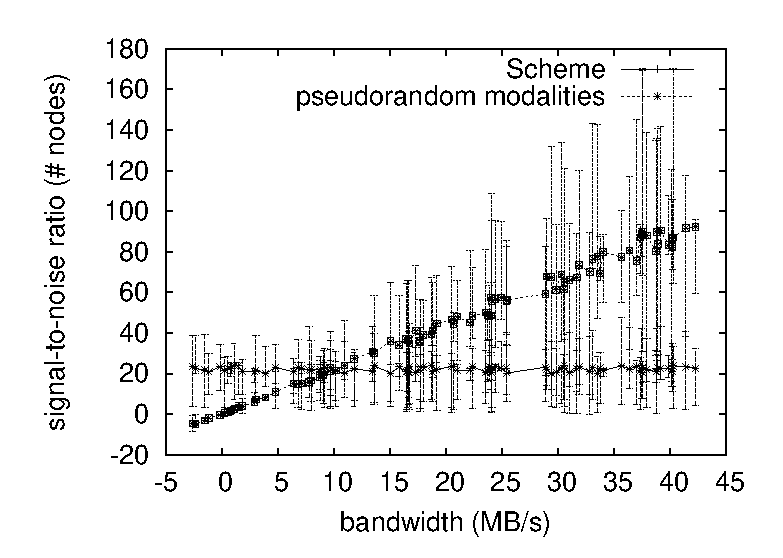
\includegraphics[width=0.4\textwidth]{figs/figure1}
\caption{상위 5개 모델 - Validation}
\label{fig:TOP5Validation}
\end{figure}
\index{figure}

\begin{figure}[!ht]
\centering
\includegraphics[width=0.4\textwidth]{figs/figure2}
\caption{상위 5개 모델 - Test}
\label{fig:TOP5Test}
\end{figure}
\index{figure}

예측 정확도 평균을 기준으로 따졌을 때, 그림~\ref{fig:TOP5Validation} 에서 가장 좋은 조합은 3번째인 [200, 300, 5, 64, 10, 64]로 설정된 모델이며, 그림~\ref{fig:TOP5Test} 에서 가장 좋은 조합은 4번째인 [200, 300, 10, 64, 10, 128]로 설정된 모델이다. 일반화하기 가장 좋은 기준으로는  [200, 300, 10, 64, 10, 128] 조합이 가장 성능이 좋은 모델이라는 것을 알 수 있다. 이는 \ref{search}에서 나타난 결과와 동일하다.

신뢰 구간을 나눠서 예측 정확도에 대한 오차 범위를 보았을 때, 5개 모델 모두 일관된 예측 정확도를 보이고 있다. 이를 통해 대부분의 모델들은 각 무작위 데이터들을 통해 잘 학습되었으며, 유형 분별에서 대체로 높은 정확도를 보인다는 것을 알 수 있다. 이에 관한 상세한 수치는 표~\ref{summary}에 나타나 있다.

\section{결 론}
이 논문에서는 대학수학능력시험 중 생명과학1 과목의 문제 5,000개의 텍스트 데이터를 가지고 5개의 유형으로 분류하는 모델을 만들고자 하였다.

Train-Validation-Test Split 형태로 6:2:2의 비율로 무작위 데이터셋을 형성하여, 6개의 하이퍼파라미터 범주를 각각 세 구간으로 나누어 Grid-Search Algorithm을 통해 729개의 서로 다른 조합 후보군을 만들었다. 형성된 조합들의 각 범주들의 예측 정확도를 평균과 표준편차로 나타내었으며, 각 범주와 예측 정확도 사이 간의 비례 관계 여부 판단과 그 원인에 대해 추정하고자 하였다.

그 다음에는, 전 실험에서 가장 높은 정확도를 나타낸 상위 조합 5개에 대한 샘플 모델을 각각 100개씩 생성하여, 각 조합 별로 예측 평균 정확도와 표준편차를 구하였다. Standard-Normal-Distribution을 통해 유의 수준을 0.01, 0.05, 0.10으로 나누어 그 오차 구간을 구하고자 하였으며, 어떤 조합의 성능이 가장 좋은지 알 수 있었다.

이미 학습된 데이터 검사를 통해 가장 높은 점수를 받은 하이퍼파라미터는 [200, 300, 5, 64, 10, 64]이며, 학습되지 않은 데이터 검사를 통해 가장 높은 점수를 받은 하이퍼파라미터는 [200, 300, 10, 64, 10, 128]이다.

결론적으로, 학습된 유형 분류 모델에서는 20 문제 중 19개의 꼴로 적절한 유형으로 나눌 수 있음을 알 수 있다. CNN 모델의 간단한 유형 분류에서도 텍스트 중심 데이터 학습으로부터 약 93.71\%라는 대체로 높은 정확도를 보였다. 추후의 연구로는 더 많은 텍스트 데이터가 쌓였을 경우와 어떠한 한 문제에 존재하는 모든 텍스트 데이터를 가져올 경우들에 대한 최적의 하이퍼파라미터 조합을 가진 모델 개발 연구도 필요해보인다.

\bibliographystyle{ieeetr}
\bibliography{ref}

\end{document}
